\documentclass{article}

%\usepackage{ragged2e}
\usepackage{graphicx}
\usepackage{amsmath}
\usepackage{siunitx}
%\usepackage{hyperref}

% for \mathbb
\usepackage{amssymb}

% This stuff is for figures, don't copy-paste
\usepackage{float}
%\DeclareGraphicsExtensions{.png, .pdf}
\DeclareGraphicsExtensions{.pdf, .png}

\renewcommand{\c}[1]{\texttt{#1}}

\begin{document}

%\begin{flushright}
    \noindent
    Rodrigo Becerril Ferreyra\\
    E E 381 Section 12\\
    Lab 3\\
    14 October 2020
%\end{flushright}

\addcontentsline{toc}{section}{Introduction}
\section*{Introduction} The purpose of this lab is to compare
an experimental set of results with the predicted binomial
distribution and Poisson distribution. A trial
is defined as
rolling three (unfair) die. A success is defined as
rolling a 1 for the first die, a 2 for the second die, and a
3 for the third die. An experiment is defined as \num{1000}
trials; the random variable \(X\) is the result of this experiment.
The probability vector is given as follows:
\begin{equation*}
    \rho = [0.2, 0.1, 0.15, 0.3, 0.2, 0.05]
\end{equation*} where the \(n\text{th}\) element of \(\rho\)
is the probability of rolling an \(n\) on the six-sided die:
for example, the probability of rolling a \num{1} on this die
is \num{0.2}.

Our trials are Bernoulli trials, since one trial does not
affect the next.
The raw output of the code
(amount of time the Problems took)
is available at the end.

\section{Problem 1} This problem has us run the experiment
(as defined above) \num{10000} times. This means that I
generated a list of \num{10000} \(X\)s. I then ploted these
on a stem plot representing the PMF of \(X\) below.
Note that this simulation took about \SI{75.7}{s}.

\begin{figure}[H]
    \centering
    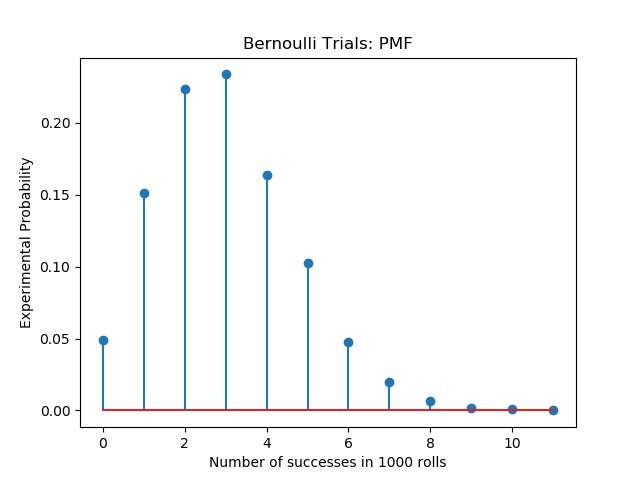
\includegraphics[height=162pt]{Images/Figure_1}
    \caption{The Probability Mass Function of \(X\).}
    \label{prob1}
\end{figure}

\section{Problem 2}
\subsection{Question} The purpose of this problem is to find the
binomial distribution regarding this problem. The binomial
distribution function is defined as follows:
\begin{equation*}
    P_b(X = x) = \binom{n}{x}p^xq^{n-x}
\end{equation*} where \(X\) is the number of successes in \(n\)
trials, \(p\) is the probability of a success, and
\(q = 1 - p\). Plotting the results for \(x = 0, 1, \ldots, 11\)
should give us a plot that is equal (or very close to) our
experiment, because our trials were Bernoulli trials.

\subsection{Results} For our trial, a success is defined
as rolling a 1, then a 2, then a 3. With the probability
vector \(\rho\) as defined above, this gives
\begin{align*}
    p &= 0.2 \times 0.1 \times 0.15 = 0.003 \\
    q &= 1-p = 0.997\\
    n &= 1000
\end{align*} Thus, our function becomes
\begin{equation*}
    P_b(X = x) = \binom{1000}{x} \left(\frac{3}{1000}\right)^x \left(\frac{997}{1000}\right)^{1000-x}
\end{equation*}

Plotting \(P_b\) gives the following plot.

\begin{figure}[H]
    \centering
    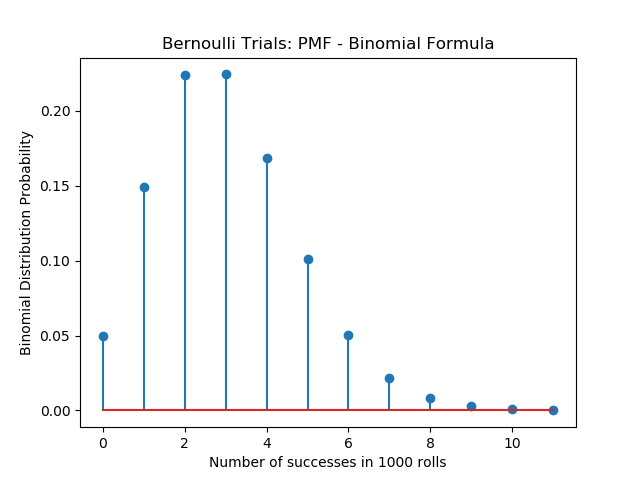
\includegraphics[height=162pt]{Images/Figure_2}
    \caption{The Binomial Distribution of \(X\).}
    \label{prob2}
\end{figure}

As it is evident, Figures \ref{prob1} and \ref{prob2} are
very similar; the difference in values is minimal and they
are almost the same. The basic shape is the same as well.
Note that this simulation took about \SI{1.98}{ms}.

\section{Problem 3}
\subsection{Question} The purpose of this problem is to see
how well a Poisson distribution can approximate a binomial
distribution. Spielgel el al. define the Poisson
distribution to be a ``good approximation'' of the binomial
distribution if the number of trials \(n \ge 50\) and
the probability \(p\) is close to zero (or \(np \le 5\)).
In this example, \(n = \num{1000} \ge 50\) and
\(np = 3 \le 5\), so a Poisson distribution is a good
approximation.

The function for the Poisson distribution is as follows:
\begin{equation*}
    P_P(X = x) =
    \begin{cases}
        \alpha^x \exp(-\alpha)/x! & \text{if } x \in \mathbb{Z}^{+}_0\\
        0 & \text{otherwise}
    \end{cases}
\end{equation*} where \(X\) denotes the number of success
in \(n\) trials, \(\alpha = np\), and \(\mathbb{Z}_0^{+}
\equiv \mathbb{Z}^{+} \cup \{0\}\) is the set of all positive
integers and zero.

\subsection{Results} Plugging in the values for \(\alpha\),
below is the Poisson distribution function that approximates
the binomial distribution.
\begin{equation*}
    P_P(X = x) =
    \begin{cases}
        3^x/e^3x! & \text{if } x \in \mathbb{Z}^+_0\\
        0 & \text{otherwise}
    \end{cases}
\end{equation*} Plotting \(P_P\) provides the following plot.

\begin{figure}[H]
    \centering
    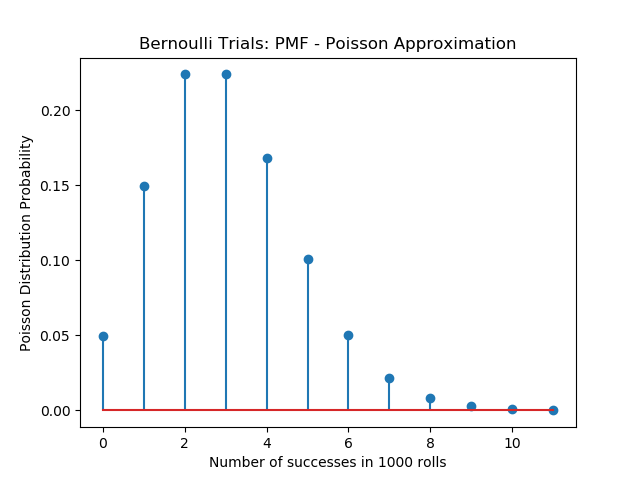
\includegraphics[height=162pt]{Images/Figure_3}
    \caption{The Poisson Distribution of \(X\).}
    \label{prob3}
\end{figure}

As is evident, the plot for this function is extremely
close to that of the binomial distribution plot. Unless one
were to compare the two plots side-by-side, it would be hard
for him or her to differentiate between the two. This
simulation took a fraction of the time as Problem 2,
at around \SI{494}{\micro\second}; that's four times as fast;
and it should be noted that on some occasions, the output
time was \SI{0}{s}. Therefore, the Poisson distribution
is a good approximation to the binomial distribution
for less resources.

\pagebreak

\section{Media} Below is the three plots for quick reference,
as well as the raw output of the source file that produced these
plots. Note that these graphics are vectors, so feel free
to zoom in (if viewing the PDF file).

\noindent
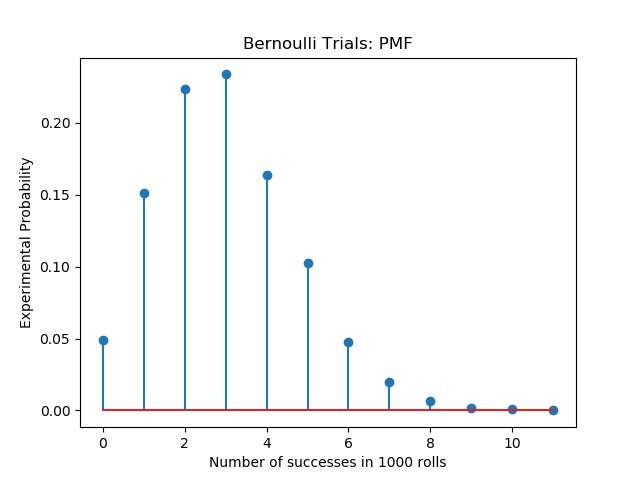
\includegraphics[width=172.5pt]{Images/Figure_1}
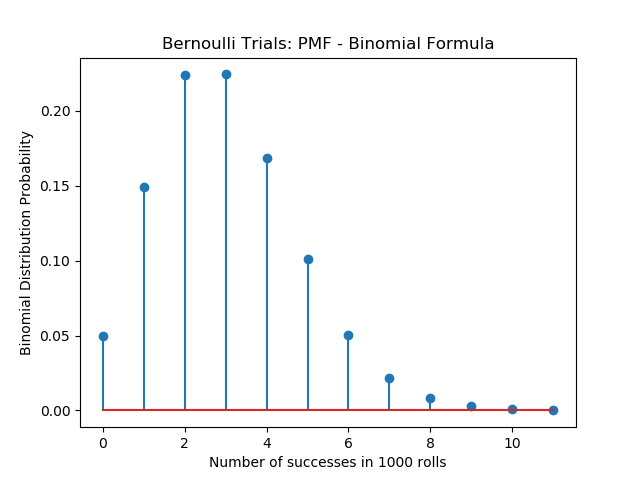
\includegraphics[width=172.5pt]{Images/Figure_2}
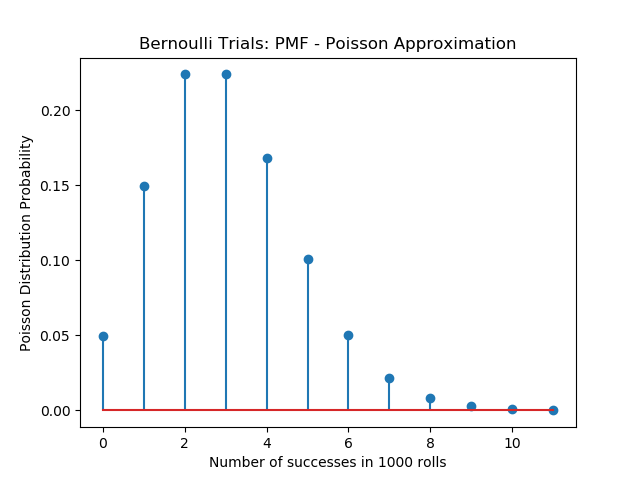
\includegraphics[width=172.5pt]{Images/Figure_3}

\begin{figure}[H]
    \centering
    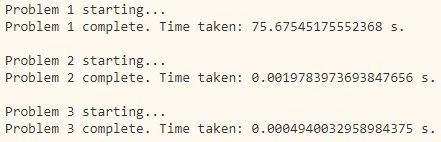
\includegraphics{Images/output}
    \caption{Output of \c{main.py}.}
    \label{output}
\end{figure}

\end{document}
